\section{Managing Project Groups} %Jeg skriver kun om admin funktionalitet her -Mikael ~♥
\todo{synes I der burde være et billede at edit siden? hvad med siden med listen?}
Before any project group can be useful it has to be created first.
Administrators need to have the ability to add, edit, and delete project groups.
The administration tools we provide have to be easy and fast to use, since they potentially have to be used many times.
This section describes how we implement the administration tools needed to manage project groups.

The features we provide to manage project groups are known as administration tools in Moodle and can be accessed through the site administration menu as seen in \figref{fig:navigation}.

\begin{figure}[htb]
	\centering
		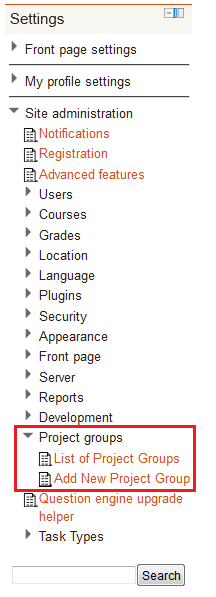
\includegraphics[scale=0.75]{images/admin-navigation.png}
	\morscaption{The settings block, which contains the site administration menu} 
	\label{fig:navigation}
\end{figure}

From here we provide a link to a list of all project groups and a link to a page, from where a new project group can be created.
The page with the list of all project groups has a table with three columns: Short name, Full name, and Actions.
As the name indicates Short name is a short name for a group. 
The Short name also serves as a link to the project group page described in \secref{sub:page}.
In the Actions column there are links to delete and edit the project group.

The edit page has the same source files as the add page.
The only difference between editing a group and adding a group is that when editing a group a HTTP parameter, $id$, is set.
When $id$ is set the form fields are filled with the relevant information from the database.
Once the submit button is pressed the function \fu{save\_or\_update\_projectgroup} is called with a project group object as input.
That function checks if the $id$ of the group is set. 
If it is we know that a project group is being edited, and we can update a row in the database.
If not we know that a new project group is being created and we insert a row in the database.

In the aforementioned list of project groups we provide a filtering functionality, which makes it easy to find a specific set of project groups.
The project group filtering is a rework of the user filtering, which already exists in Moodle.
This functionality is requested by the administrative personnel (see \secref{sec:requirements}).
